\input{preamble}
\input{format}
\input{commands}
\usepackage{graphicx}


\begin{document}

\begin{Large}
    \textsf{\textbf{Feb 19. 2026}}
    
    Left to their own devices
\end{Large}

\vspace{1ex}

\textsf{\textbf{Observer:} Aiden Thomas}\\
\textsf{\textbf{Teacher:} Eric Baez}


\vspace{2ex}
Reflections on Classroom Observation

\hspace{2ex} This week, Eric continued to provide me with a comprehensive set of student expectations, which outlined the submission criteria required for the AP Computer Science Principles (APCSP) program. A challenge I faced today was that some students already submitted, so they were not interested in anything really and were looking for wallpapers. As a result, I taught them the Russian Card game \texttt{Durak}, I noticed a meaningful overlap between the two courses and thought they might want to build a card game as another portfolio submission, as students would draw upon programming techniques and tools introduced in Video Game Design to fulfill their APCSP portfolio requirements. This highlighted the natural transferability of skills, even when the work extends beyond the boundaries of the original curriculum.


\begin{figure}[h!]

\begin{problem}{Adaptability}{problem-label}
    \begin{enumerate}[(a)]
        \item Below is an image of Durak.
    
        \begin{center}
            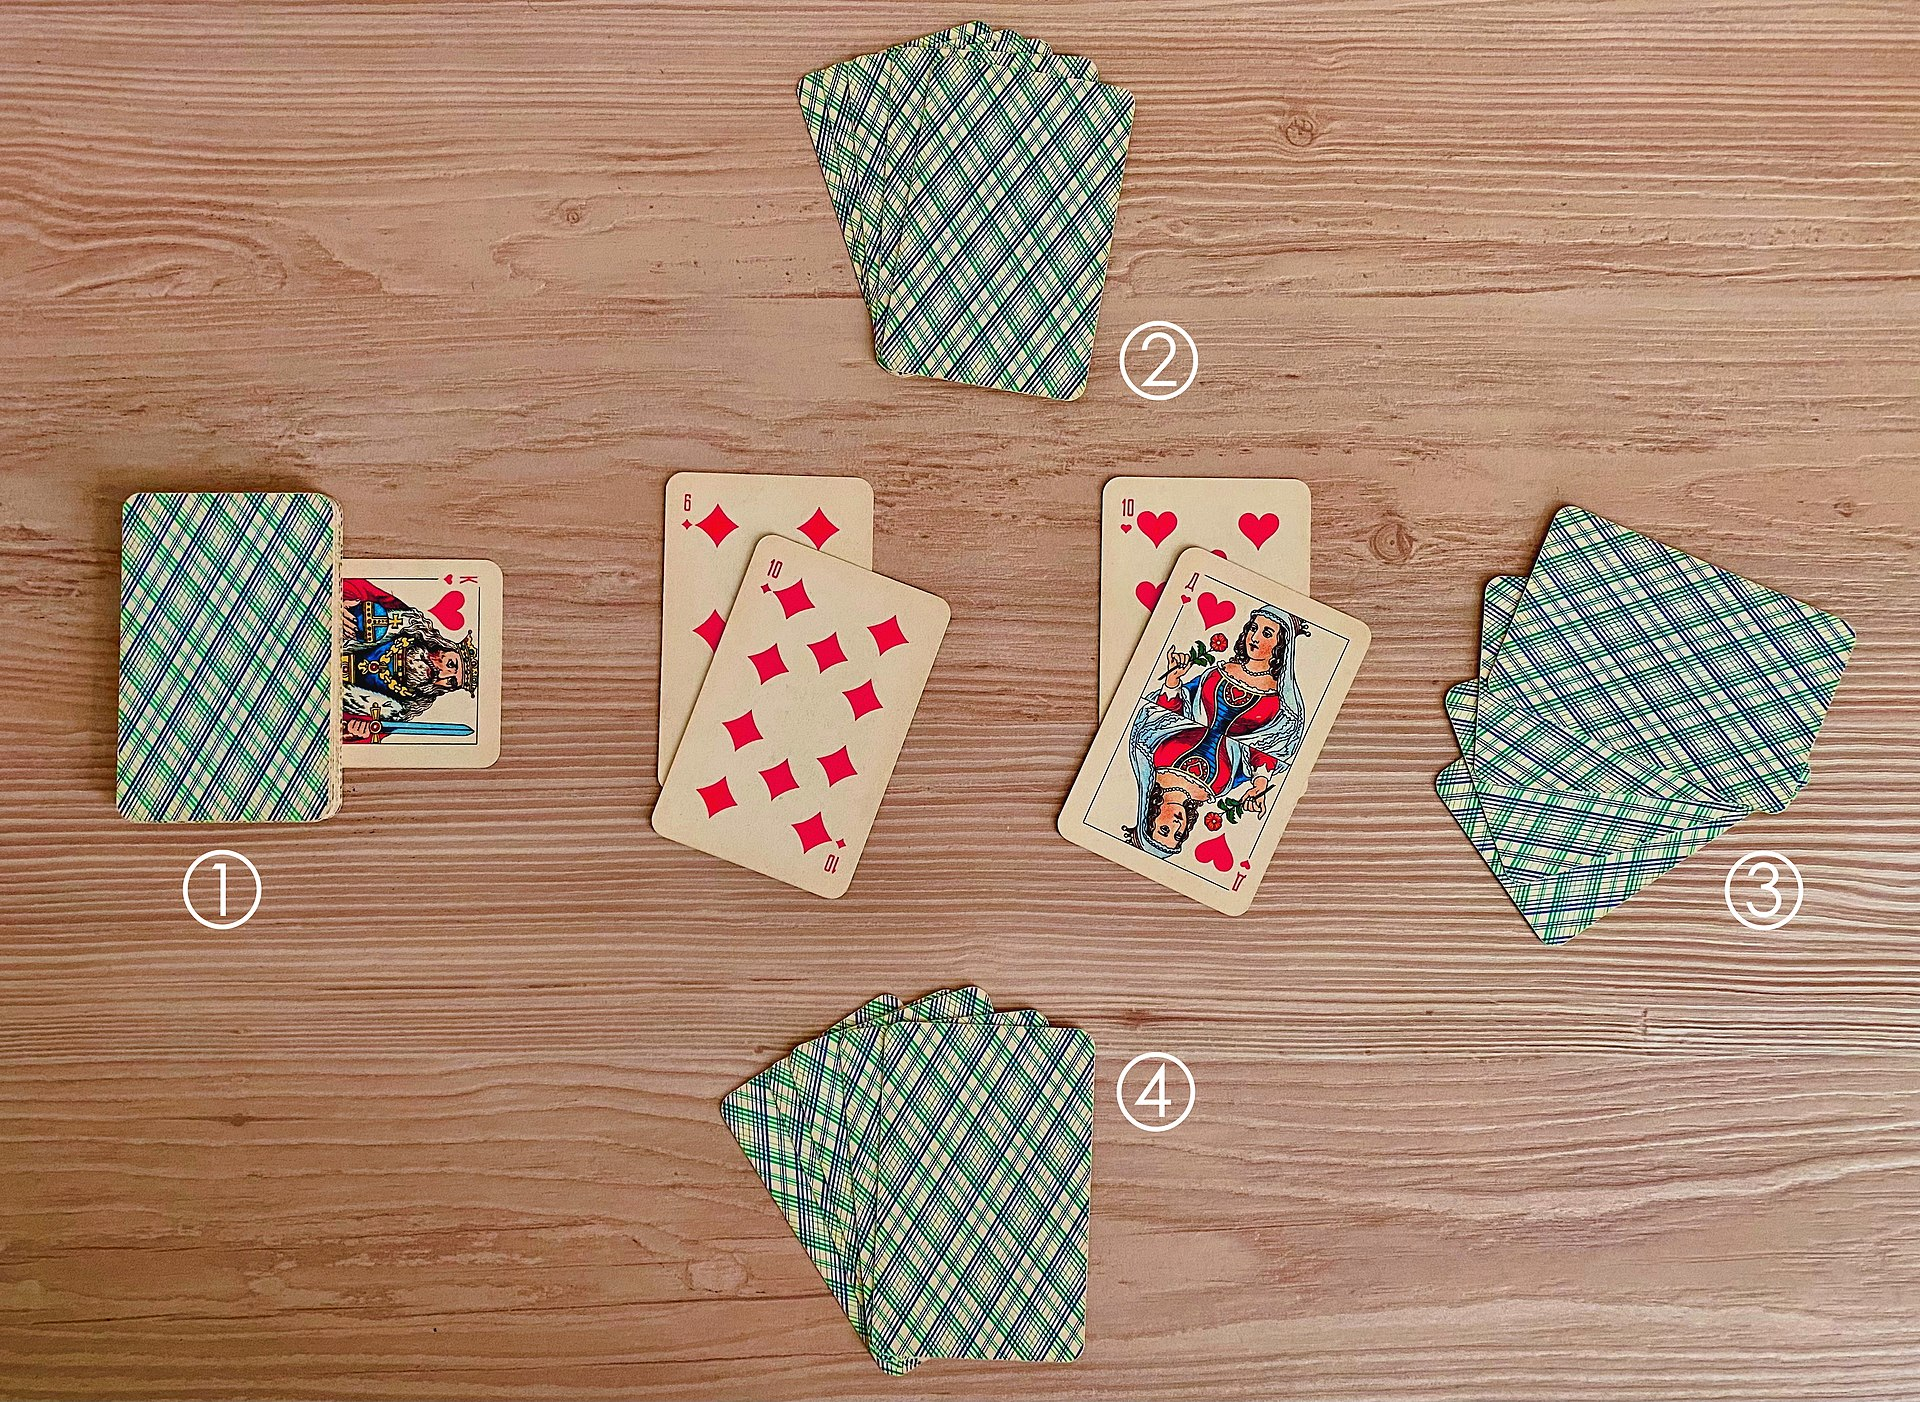
\includegraphics[width=0.5\linewidth]{example.jpg}
            \label{fig:boat1}
        \end{center}
    \end{enumerate}
\end{problem}

\end{figure}


% =================================================

\hspace{2ex} Moving forward, I intend to refine my approach to assignment design and structure, ensuring that tasks are more accessible and relevant to students who are just beginning their journey with computer science.
\vspace{2ex}
\hspace{2ex} Comfortability: \textbf{7/10}\
\hspace{2ex} I selected this rating because I recognize that I still need to recalibrate my expectations when working with students who have had significantly less exposure to programming compared to those at the college level.

\bibliographystyle{apalike}

\end{document}
